\documentclass{amia}
\usepackage{graphicx}
\usepackage[labelfont=bf]{caption}
\usepackage[superscript,nomove]{cite}
\usepackage{color}


\begin{document}


\title{A framework for quality in inner-sourced R packages and Shiny dashboards}

\author{James A. Black, PhD^{1}$, Adam J. Foryś, PhD^{2}$}

\institutes{
    $^1$PD Personalised Healthcare, Roche; $^2$7N Consulting\\
}

\maketitle

\noindent{\bf Abstract}

\textit{Abstract text goes here, justified and in italics.  The abstract would normally be one paragraph long.  See Table 1. for appropriate abstract length by submission type.}

\section*{Introduction}
This template should be used as a starting point for AMIA submissions.  
It is important to review the AMIA Call for Participation (CFP) where types of submissions considered and general requirements for each submission type are listed. All submissions must conform to the format and presentation requirements described in the CFP and at the submission site.


\section*{Another Major Heading and References}
This sentence has two reference citations\cite{ref1,ref2}.

More text of an additional paragraph, with a figure reference (Figure ~\ref{fig1}) and a figure inside a Word text box below.  Figures need to be placed as close to the corresponding text as possible and not extend beyond one page.\\
\begin{figure}[h!]
\centering
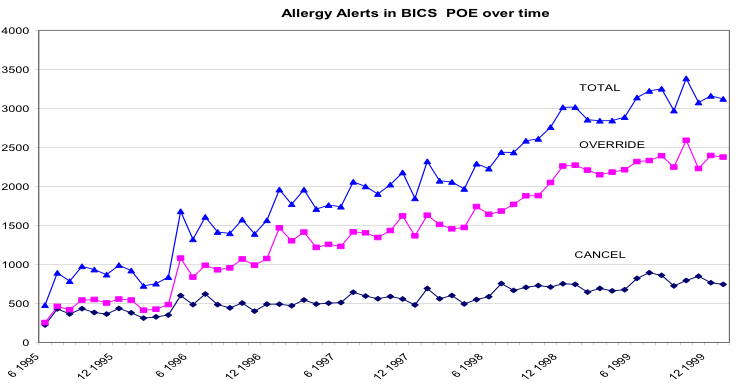
\includegraphics[scale=1]{pics/figure1.png}
\caption{Total allergy alerts, overridden alerts, or drug order cancelled.}
\label{fig1}
\end{figure}

This is additional text added just to show the one-column formatting.  This is additional text added just to show the one-column formatting.  This is additional text added just to show the one-column formatting.  This is additional text added just to show the one-column formatting.  This is additional text added just to show the one-column formatting.  This is additional text added just to show the one-column formatting.  This is additional text added just to show the one-column formatting.

This paragraph contains a reference to a table just below (Table 1).  All tables need to be placed as close to the corresponding text as possible, But each individual table should be on one page and not extend to multiple pages unless labeled as ``��Continued"��.

\begin{table}[h]
\centering
\caption{Submission type, abstract length, and page length maximum for AMIA submissions.}
  \begin{tabular}{|l|l|l|}
  \hline
    \textbf{Submission Type}    & \textbf{Abstract Length}  & \textbf{Page Length Maximum**} \\ \hline
    Paper  & 125-150 words  & Ten   \\ \hline
    Student Paper  & 125-150 words  & Ten \\ \hline
    Poster  &50-75 words*   & One \\ \hline
    Podium  Abstract & 50-75 words*  & Two \\ \hline
    Panel   &150-200 words  & Three \\ \hline
    System Demonstrations    &150-200 words  & One \\ \hline
  \end{tabular}
\end{table}
*: All podium abstract and poster submissions must have a brief (50-75 words) abstract. The abstract does NOT have to be part of the document, but must be entered on the submission website in the Abstract box in Step 2.

**: \textcolor{red}{If your submission is longer than what is specified below, it will be rejected without review.}

This is another paragraph.

\section*{Conclusion}
Your conclusion goes at the end, followed by References, which must follow the Vancouver Style (see: www.icmje.org/index.html).  References begin below with a header that is centered.  Only the first word of an article title is capitalized in the References. 

\makeatletter
\renewcommand{\@biblabel}[1]{\hfill #1.}
\makeatother



\bibliographystyle{unsrt}
\begin{thebibliography}{1}
\setlength\itemsep{-0.1em}

\bibitem{ref1}
Pryor TA, Gardner RM, Clayton RD, Warner HR. The HELP system. J Med Sys. 1983;7:87-101.
\bibitem{ref2}
Gardner RM, Golubjatnikov OK, Laub RM, Jacobson JT, Evans RS. Computer-critiqued blood ordering using the HELP system. Comput Biomed Res 1990;23:514-28.



\end{thebibliography}

\end{document}